%!TEX root = ./Basilisk-spacecraft-20170808.tex

\section{Test Description and Success Criteria}
This test is located in \texttt{simulation/dynamics/spacecraftDynamics/\_UnitTest/\newline
test\_multiSpacecraft.py}. 

\subsection{SCConnected Test}
This test ensures that a spacecraft system with hingedRigidBodies attached to it conserves energy and momentum.

\section{SCConnectedAndUnconnected Test}
This test ensures that a spacecraft system with hingedRigidBodies attached to it and other unconnected spacecraft can be simulated at the same time and conserve energy and momentum.

\section{Test Results}

\subsection{SCConnected Test}
\begin{figure}[htbp]
	\centerline{
		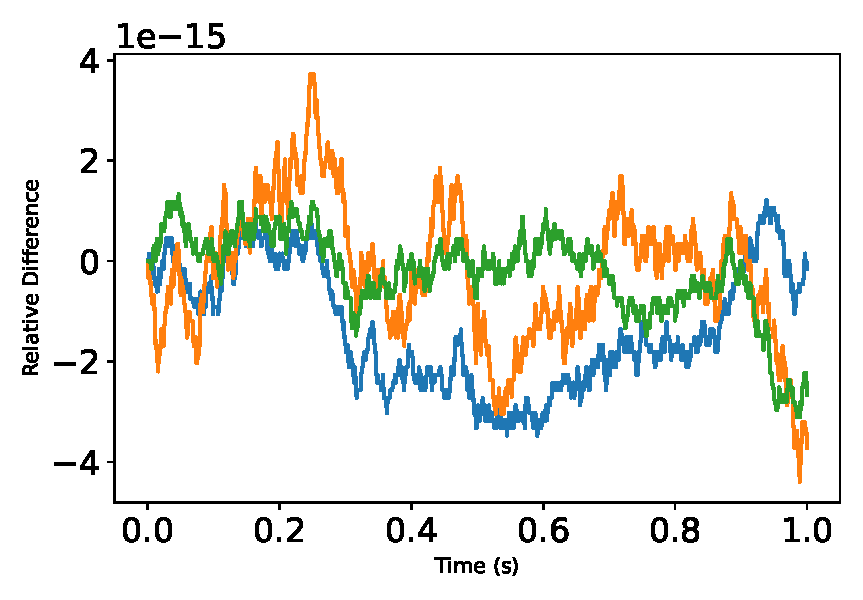
\includegraphics[width=0.8\textwidth]{../AutoTeX/ChangeInOrbitalAngularMomentumSystem}}
	\caption{Change in Orbital Angular Momentum System with Gravity}
	\label{fig:ChangeInOrbitalAngularMomentumSystem}
\end{figure}

\begin{figure}[htbp]
	\centerline{
		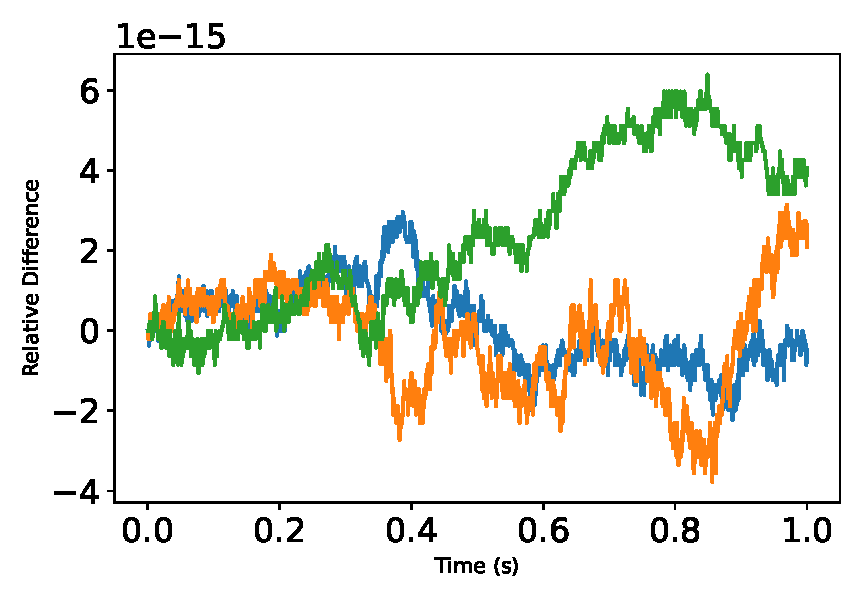
\includegraphics[width=0.8\textwidth]{../AutoTeX/ChangeInRotationalAngularMomentumSystem}}
	\caption{Change In Rotational Angular Momentum System with Gravity}
	\label{fig:ChangeInRotationalAngularMomentumSystem}
\end{figure}

\begin{figure}[htbp]
	\centerline{
		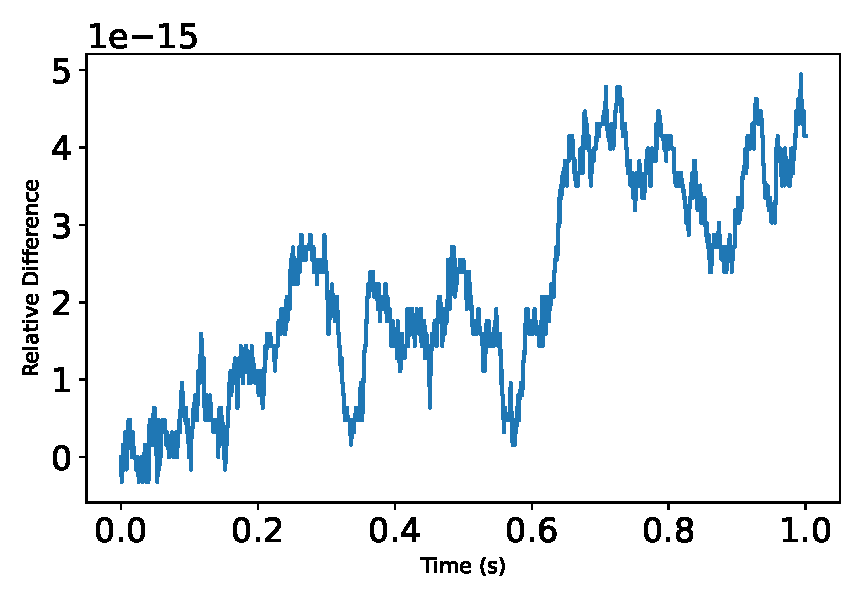
\includegraphics[width=0.8\textwidth]{../AutoTeX/ChangeInRotationalEnergySystem}}
	\caption{Change In Rotational Energy System with Gravity}
	\label{fig:ChangeInRotationalEnergySystem}
\end{figure}

\begin{figure}[htbp]
	\centerline{
		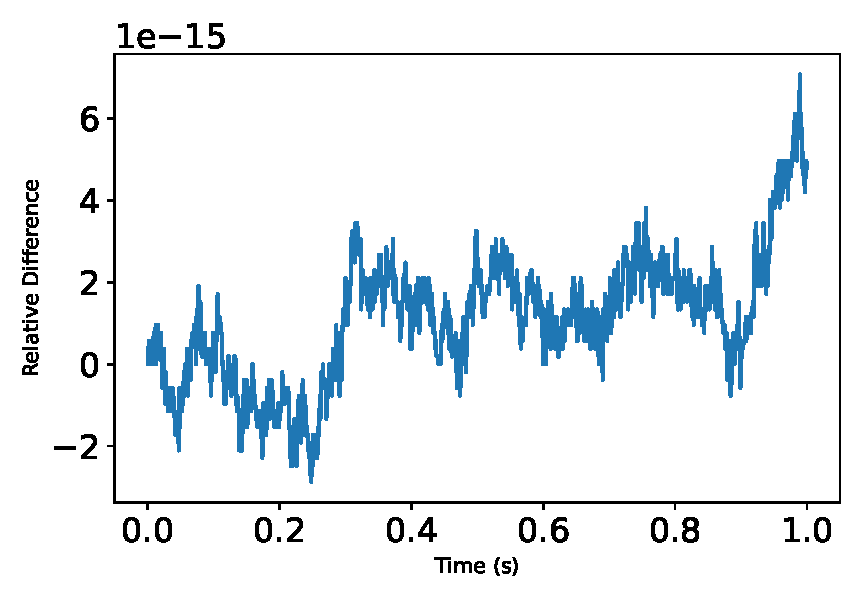
\includegraphics[width=0.8\textwidth]{../AutoTeX/ChangeInOrbitalEnergySystem}}
	\caption{Change in Orbital Energy System with Gravity}
	\label{fig:ChangeInOrbitalEnergySystem}
\end{figure}

\clearpage

\subsection{SCConnectedAndUnconnected Test}

\begin{figure}[htbp]
	\centerline{
		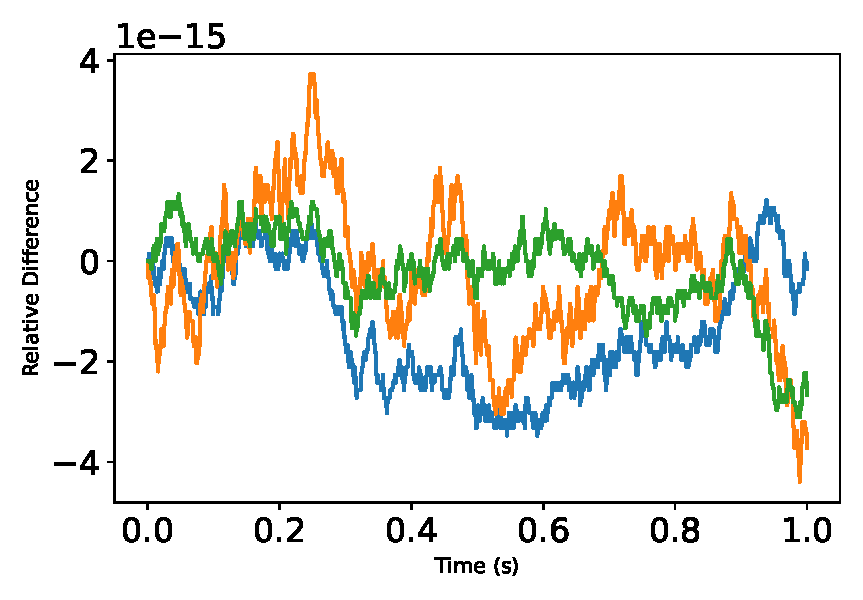
\includegraphics[width=0.8\textwidth]{../AutoTeX/ChangeInOrbitalAngularMomentum}}
	\caption{Change in Orbital Angular Momentum System with Gravity}
	\label{fig:ChangeInOrbitalAngularMomentum}
\end{figure}

\begin{figure}[htbp]
	\centerline{
		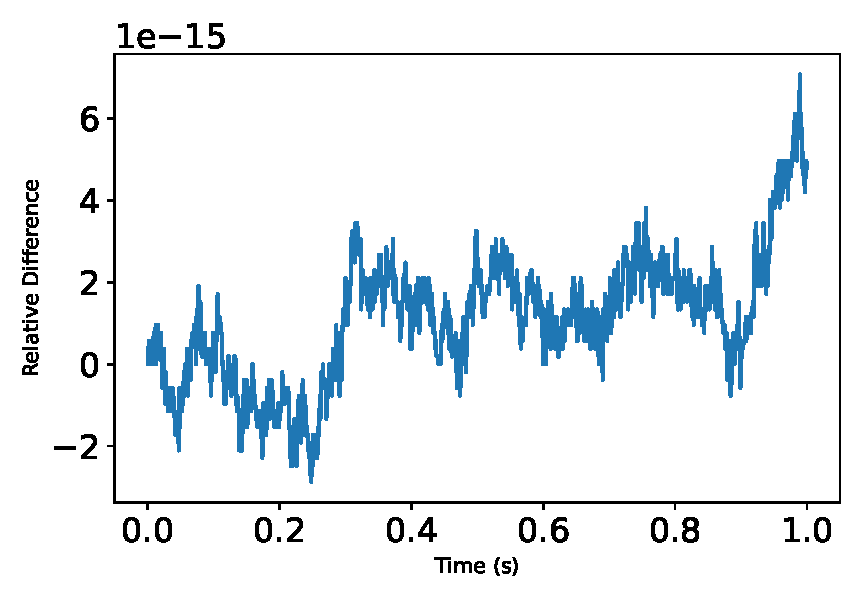
\includegraphics[width=0.8\textwidth]{../AutoTeX/ChangeInOrbitalEnergy}}
	\caption{Change in Orbital Energy System with Gravity}
	\label{fig:ChangeInOrbitalEnergy}
\end{figure}

\begin{figure}[htbp]
	\centerline{
		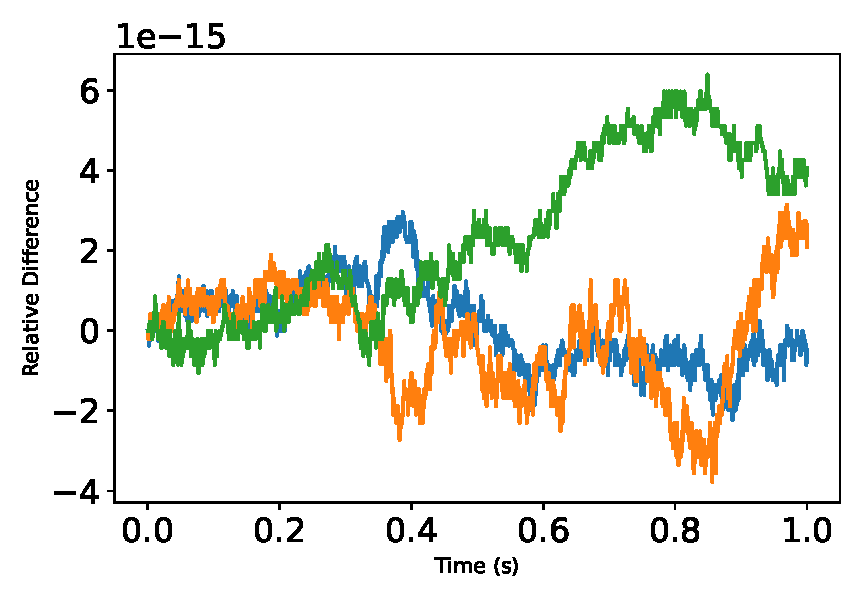
\includegraphics[width=0.8\textwidth]{../AutoTeX/ChangeInRotationalAngularMomentum}}
	\caption{Change In Rotational Angular Momentum System with Gravity}
	\label{fig:ChangeInRotationalAngularMomentum}
\end{figure}

\begin{figure}[htbp]
	\centerline{
		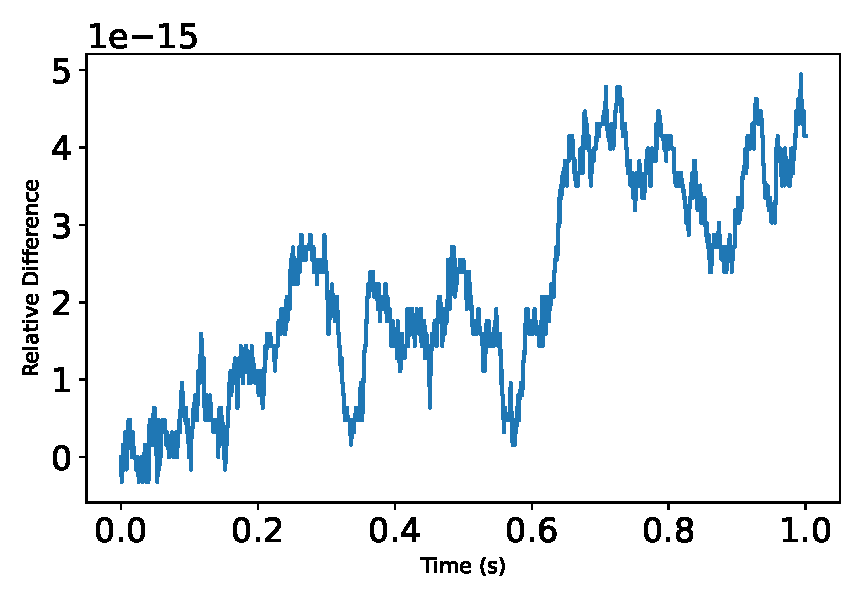
\includegraphics[width=0.8\textwidth]{../AutoTeX/ChangeInRotationalEnergy}}
	\caption{Change In Rotational Energy System with Gravity}
	\label{fig:ChangeInRotationalEnergy}
\end{figure}

\begin{figure}[htbp]
	\centerline{
		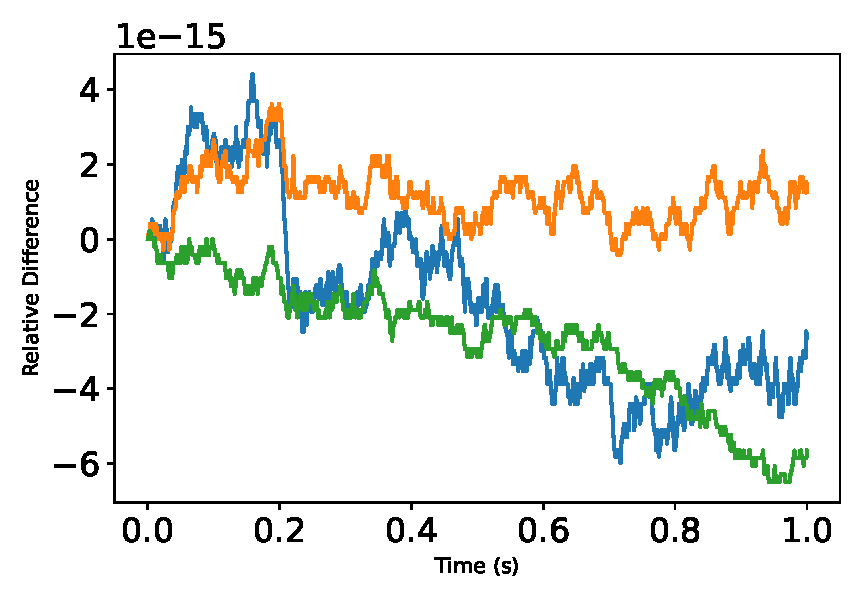
\includegraphics[width=0.8\textwidth]{../AutoTeX/ChangeInOrbitalAngularMomentum1}}
	\caption{Change in Orbital Angular Momentum SC 1 with Gravity}
	\label{fig:ChangeInOrbitalAngularMomentum1}
\end{figure}

\begin{figure}[htbp]
	\centerline{
		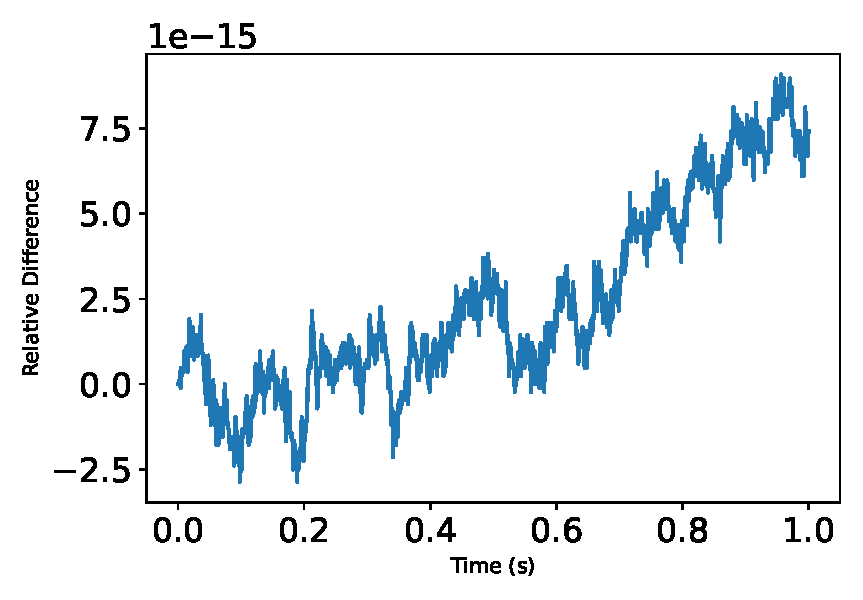
\includegraphics[width=0.8\textwidth]{../AutoTeX/ChangeInOrbitalEnergy1}}
	\caption{Change in Orbital Energy SC 1 with Gravity}
	\label{fig:ChangeInOrbitalEnergy1}
\end{figure}

\begin{figure}[htbp]
	\centerline{
		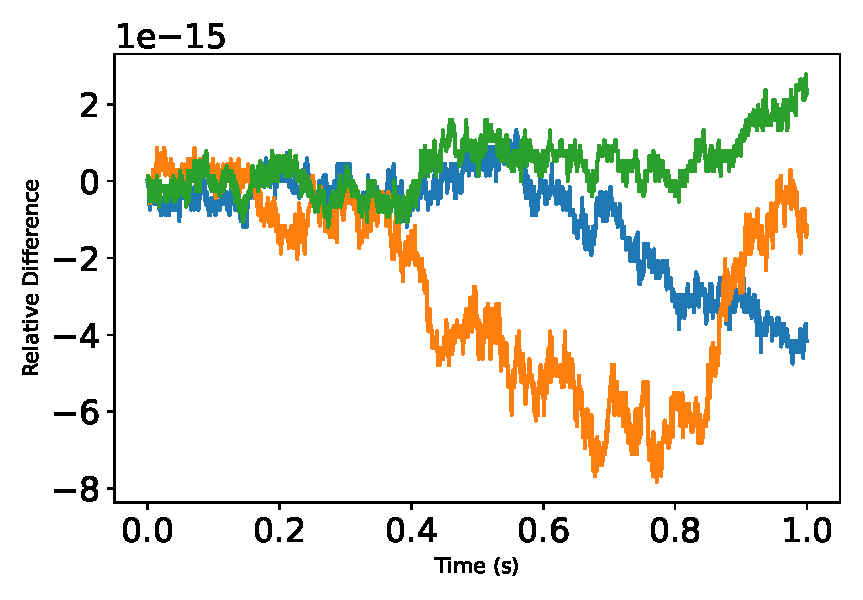
\includegraphics[width=0.8\textwidth]{../AutoTeX/ChangeInRotationalAngularMomentum1}}
	\caption{Change In Rotational Angular Momentum SC 1 with Gravity}
	\label{fig:ChangeInRotationalAngularMomentum1}
\end{figure}

\begin{figure}[htbp]
	\centerline{
		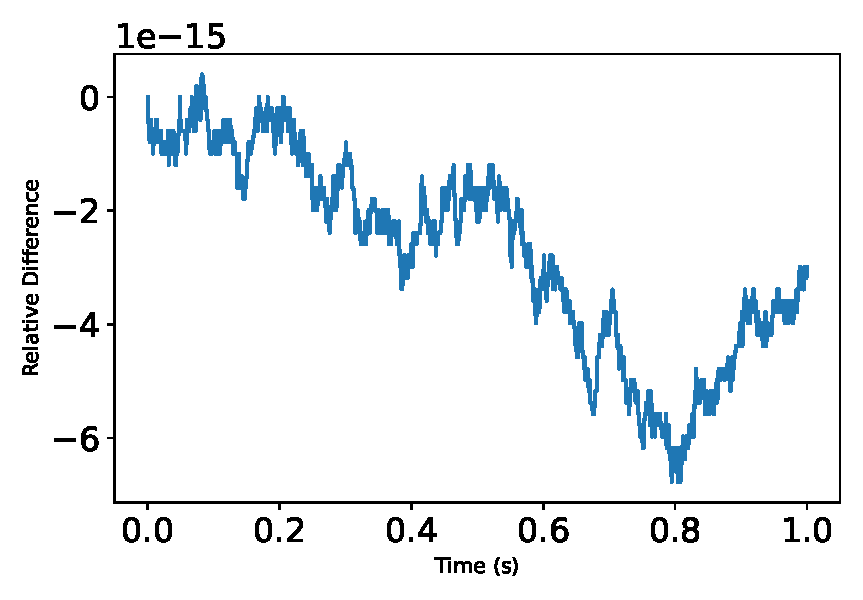
\includegraphics[width=0.8\textwidth]{../AutoTeX/ChangeInRotationalEnergy1}}
	\caption{Change In Rotational Energy SC 1 with Gravity}
	\label{fig:ChangeInRotationalEnergy1}
\end{figure}

\begin{figure}[htbp]
	\centerline{
		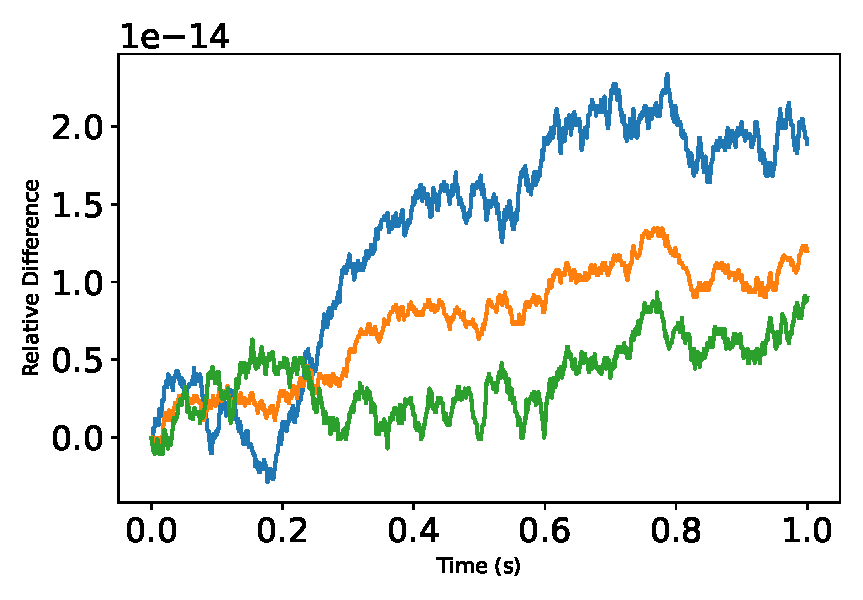
\includegraphics[width=0.8\textwidth]{../AutoTeX/ChangeInOrbitalAngularMomentum2}}
	\caption{Change in Orbital Angular Momentum SC 2 with Gravity}
	\label{fig:ChangeInOrbitalAngularMomentum2}
\end{figure}

\begin{figure}[htbp]
	\centerline{
		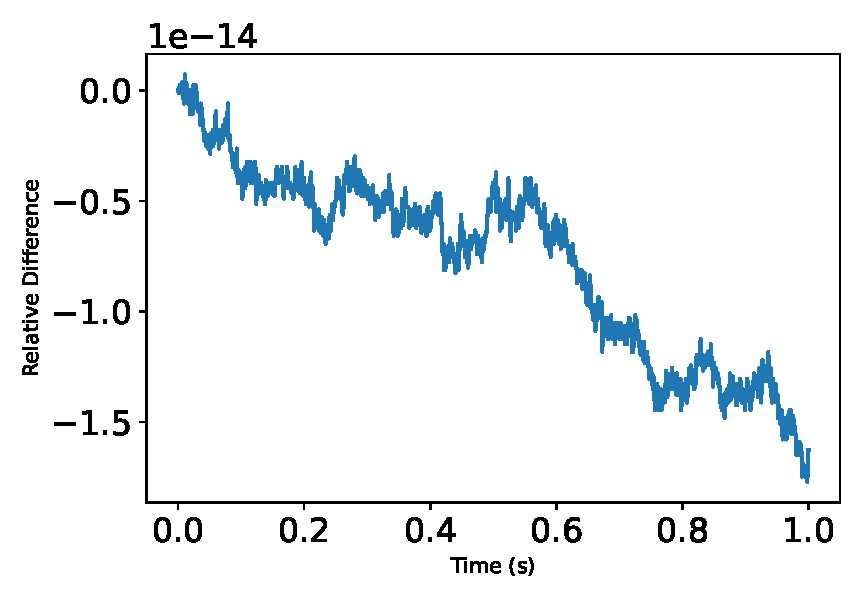
\includegraphics[width=0.8\textwidth]{../AutoTeX/ChangeInOrbitalEnergy2}}
	\caption{Change in Orbital Energy SC 2 with Gravity}
	\label{fig:ChangeInOrbitalEnergy2}
\end{figure}

\begin{figure}[htbp]
	\centerline{
		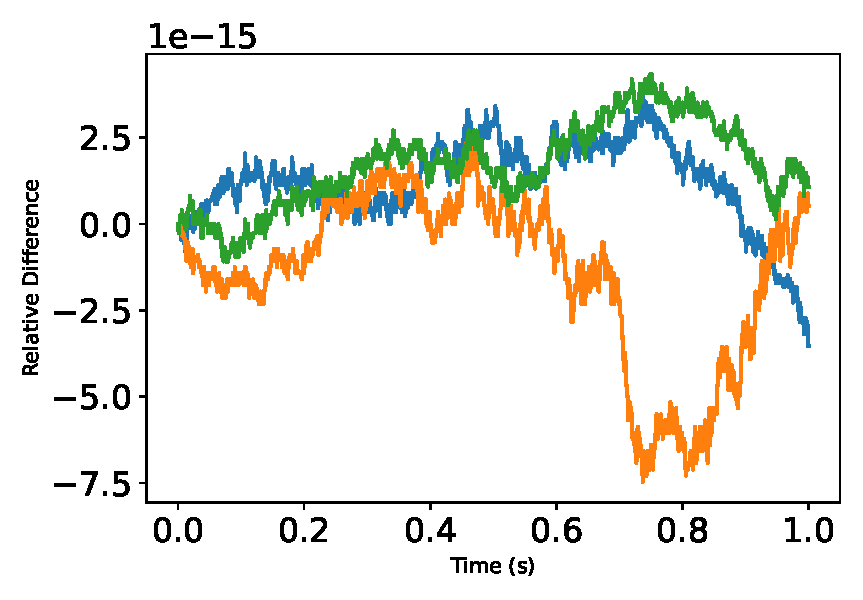
\includegraphics[width=0.8\textwidth]{../AutoTeX/ChangeInRotationalAngularMomentum2}}
	\caption{Change In Rotational Angular Momentum SC 2 with Gravity}
	\label{fig:ChangeInRotationalAngularMomentum2}
\end{figure}

\begin{figure}[htbp]
	\centerline{
		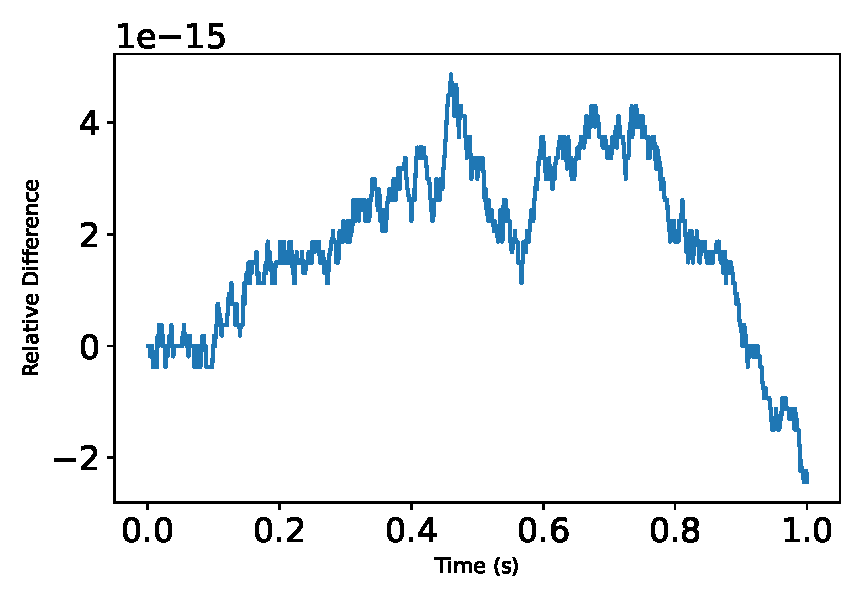
\includegraphics[width=0.8\textwidth]{../AutoTeX/ChangeInRotationalEnergy2}}
	\caption{Change In Rotational Energy SC 2 with Gravity}
	\label{fig:ChangeInRotationalEnergy2}
\end{figure}

\clearpage